\subsection{Resultados obtenidos por el prototipo a 30.00 C}

\begin{figure}[H]
	\centering
	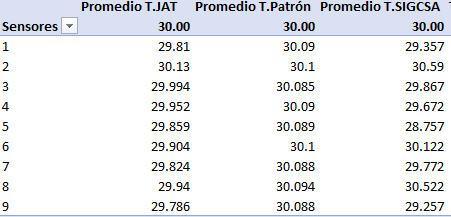
\includegraphics[width=0.5\linewidth]{resultados7.png}
	\caption{Tabla de Promedios de Temperaturas de prototipo y termómetros a 30.00 C}
\end{figure}

\par \noindent 
Los resultados obtenidos por las calibraciones, ver Anexo 4 , son utilizados para calcular la temperatura promedio del termómetro patrón, los nueve termómetros de campo de SIGCSA y los sensores de temperatura del prototipo, ver figura 4.7 y con estos valores podemos realizar la siguiente gráfica:

\begin{figure}[H]
	\centering
	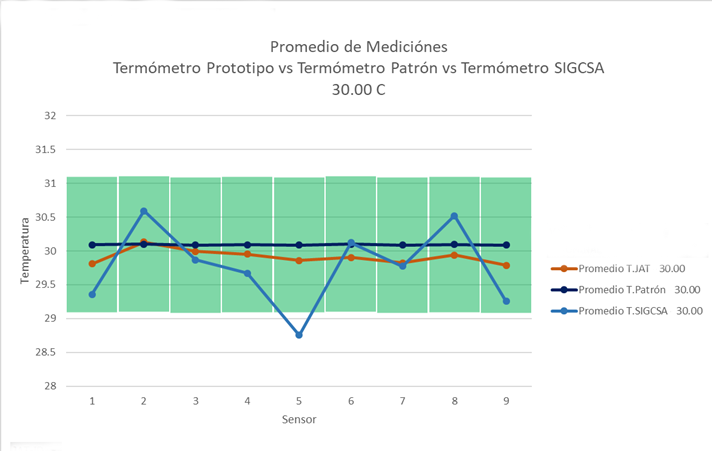
\includegraphics[width=0.6\linewidth]{resultados8.png}
	\caption{Grafica de Promedios de Temperaturas de prototipo y termómetros a 30.00 C}
\end{figure}

\par \noindent
La figura 4.8 en la gráfica el termómetro de campo de SIGCSA, el numero 5 a salido del error permitido con respecto al patrón. Adicional los termómetros 1, 2, 8 y 9 también se encuentran con un error mayor de 0.5 grados con respecto al  patrón. Esto indica que los termómetros de campo comenzarán a indicar valores de temperatura inexactos a medida que sube la temperatura del medio isotermo a calibrar. Sin embargo los sensores del prototipo aún mantienen las mismas lecturas con respecto al patrón. A continuación son los resultados a una temperatura de 50.00 grados Celsius.
